\chapter{myc2d.h,myc.h Documentation}
\ifsingle
\maketitle
\fi
\chaptermeta[draft][2025-07-15]

\section{Introduction}
‘MYC’ stands for the Mixed Young’s Centered scheme, introduced by Scardovelli et al. \cite{2003_Scardovelli}. It is used to compute the interface normal vector $\mathbf{n}$ at a given cell, based on the volume fraction $c$ in the current cell and its neighboring cells (9 cells in 2D and 27 cells in 3D).

In the following sections, I will first introduce the basic concept of representing an interface with a linear function, followed by the algorithm that enables the mixed scheme to determine the normal direction in 2D cases. This will then be extended to the 3D scenario.

\subsection{2D scenario}
\subsubsection{Linear Representation of the Interface}

Consider an interfacial cell on a 2D plane, as shown in figure \ref{fig:myc-2Dlinear}. Let the normal direction of the interface be denoted by $\mathbf{n} = (n_x, n_y)$. It is straightforward to show that the interface can be represented by the linear equation
\begin{equation}{equ:myc-original}
  n_x X + n_y Y = \alpha,
\end{equation}
where $\alpha$ is a constant that determines the position of the interface.

\begin{figure}[ht]
    \centering
    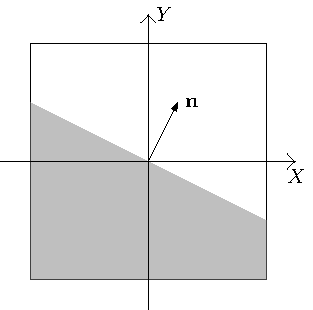
\includegraphics[height=6cm]{./image/myc-h-and-myc2d-h/2Dlinear-face.pdf}
    \caption{Linear representation of the interface, with normal direction $\mathbf{n} = (n_x, n_y)$.}
    \label{fig:myc-2Dlinear}
\end{figure}

This equation indicates that the linear interface within a cell is fully characterized once the triplet $(n_x, n_y, \alpha)$ is known.

If we treat $Y$ as a function of $X$, the equation takes the slope-intercept form
\begin{equation}\label{equ:myc-centered}
  sign(n_y)Y = -\frac{n_x}{|n_y|} X + \frac{\alpha}{|n_y|} = m_y X + b_y,
\end{equation}
where $m_y = -\frac{n_x}{|n_y|}$ and $b_y = \frac{\alpha}{|n_y|}$.

Similarly, $X$ can be expressed as a function of $Y$, with slope $m_x = -\frac{n_y}{|n_x|}$. The normal direction obtained from equation \ref{equ:myc-centered} can thus be written in the form $(-m_x,, \text{sign}(n_y))$ (or equivalently, $(\text{sign}(n_x),, -m_y)$). This form is derived by transforming equation \ref{equ:myc-centered} back into the original form of the interface representation, as shown in equation \ref{equ:myc-original}.

With the interface representation clarified, we now introduce the centered scheme, Young’s scheme, and finally the mixed scheme. As will be shown, the centered scheme estimates the interface normal direction through the form of equation \ref{equ:myc-centered}, while Young’s scheme directly computes the normal vector $(n_x, n_y)$.
\subsubsection{Centered columns scheme}

For the linear equation \ref{equ:myc-centered}, the most straightforward way to compute the slope is by selecting an arbitrary pair of points on the line, denoted as $(X_1, Y_1)$ and $(X_2, Y_2)$, and calculating  
\begin{equation}
  m_x = \frac{Y_2 - Y_1}{X_2 - X_1}.
\end{equation}  
The centered columns scheme adopts the same idea but operates under discrete conditions. This naturally raises several questions:  
\begin{enumerate}
  \item Given a value of $X$, how can we determine the corresponding output $Y$ in a discrete setting?
  \item Since there are two slope estimates, which one should be selected?
\end{enumerate}

\begin{figure}[ht]
    \centering
    \begin{subfigure}[t]{0.45\textwidth}
        \centering
        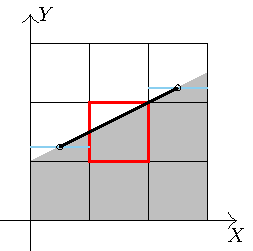
\includegraphics[height=5cm]{./image/myc-h-and-myc2d-h/centered-a.pdf}
        \subcaption{}
        \label{fig:myc-centered-a}
    \end{subfigure}
    \begin{subfigure}[t]{0.45\textwidth}
        \centering
        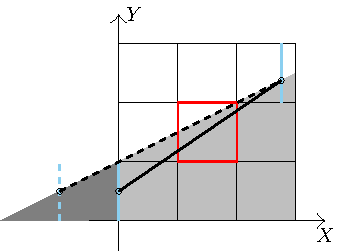
\includegraphics[height=5cm]{./image/myc-h-and-myc2d-h/centered-b.pdf}
        \subcaption{}
        \label{fig:myc-centered-b}
    \end{subfigure}
    \caption{Sketch of the computation process for the centered scheme. The red cell highlights the current cell where the interfacial slope is being computed. The blue lines represent the summation of volume fractions across columns, and the black solid line shows the resulting slope obtained by the centered scheme. In figure (a), the scheme accurately captures the interface when it spans across opposite boundaries. By contrast, figure (b) presents the same scenario but from a complementary perspective. The result reveals a significant discrepancy between the computed and actual slopes. Note that the dashed and solid lines are intentionally reversed to facilitate comparison with the true slope of the interface.}
    \label{fig:myc-centered}
\end{figure}

Figure~\ref{fig:myc-centered-a} illustrates the first question by showing how the centered scheme computes the interfacial slope. Similar to the height function method described in the \texttt{heights.h} documentation, the value of $Y$ at each column is approximated by summing the volume fractions $c$ of three adjacent cells aligned along the same $X$ coordinate. Once two neighboring values (marked as empty circles) are obtained, the slope at the current cell (highlighted in red) is computed using a centered finite difference. The result is indicated by the solid black line.

Let the current cell be denoted by index $(0, 0)$. The slope in figure~\ref{fig:myc-centered-a} is then given by:
\begin{equation}
m_x = \frac{1}{2} \left(\sum_{j=-1}^{1} c_{1,j} - \sum_{j=-1}^{1} c_{-1,j} \right)
\end{equation}

Since $m_x = -\frac{n_y}{|n_x|}$, it follows that $\text{sign}(n_x) = -\text{sign}(m_x)$, and similarly, $\text{sign}(n_y) = -\text{sign}(m_y)$. This dual representation for the same interface raises the second question: which of the two directional estimates gives the more accurate result?

Figure \ref{fig:myc-centered-b} presents the same scenario but treats $Y$ as the independent variable and $X$ as the dependent output. In this case, the slope computed by the centered scheme deviates significantly from the true interface, as part of the left column (shown in dark gray) is omitted. For a perfectly linear interface, the centered scheme yields accurate results only when the interface intersects the left and right boundaries of the current cell. However, when the interface crosses adjacent boundaries (e.g., left and top) or spans the top and bottom boundaries, the accuracy deteriorates due to partial volume loss, as illustrated in figure~\ref{fig:myc-centered-b}. In other words, the smaller the absolute value of the slope, the more accurate the estimate \cite{2007_Aulisa}.

Based on this observation, the normal direction is chosen as $(-m_x, sign(m_y))$ when $|m_y| > |m_x|$, and as $(sign(m_x), -m_y)$ otherwise.

\printbibliography

